%%%%%%%%%%%%%
%  Ch1 : Generalities  %
%%%%%%%%%%%%%

\chapter{Discrete systems}
	\section{Introduction}
		Vibrations are found on everything around us, trains, cars and even human body is subject to vibration. Its effects are disturbing because it causes fatigue, loss of performance, no comfort, ... As vibration source we can find the earthquakes, the interaction with road, the wind, the waves, ... The basic terminology for the course is:
		
		\begin{multicols}{3}
		\begin{itemize}
		\item[•] \textbf{The source} $F(\omega)$,\\
		this characterizes the dynamic forces
		\item[•] \textbf{The path} $H(\omega)$,\\
		this characterizes the structural dynamics
		\item[•] \textbf{The response} $X(\omega)$,
		such that $X(\omega)=H(\omega)F(\omega)$.
		\end{itemize}
		\end{multicols}
		
		Vibrations cause failure, loss of comfort and is harmful for precision operations. We try to suppress it by damping, isolation and structure design.\\
		
		We have two different approach for analysing a vibration problem. The one called \textbf{Signal analysis} or \textbf{Fourier analysis} deals with the case where we only have the response of the system to unknown forces. The one called \textbf{System analysis} or \textbf{Modal analysis} where we stimulate the system with known forces and measure the response, being able to find $H(s)$ (dynamic forces - transfer function of the system). \\
		
			\subsubsection{Basic notions}
			\begin{wrapfigure}[7]{l}{2.5cm}
			\vspace{-5mm}
			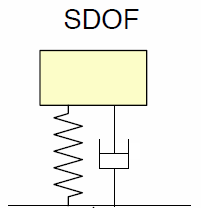
\includegraphics[scale=0.5]{ch1/1}
			\captionof{figure}{}
			\end{wrapfigure}			
			Three main forces are acting on bodies:
			
			\begin{itemize}
				\item[•] the one due to springs, proportional to the displacement: $F = kd $
				\item[•] the one due to dampers, proportional to the velocity: $F = cv$
				\item[•] the one due to the mass, proportional to acceleration: $F =ma$.
			\end{itemize}
			
			\ \\ Notice that we have one resonance frequency for each degree of liberty of each mass. \newpage
			
			\begin{wrapfigure}[8]{r}{4cm}
			\vspace{-8mm}
			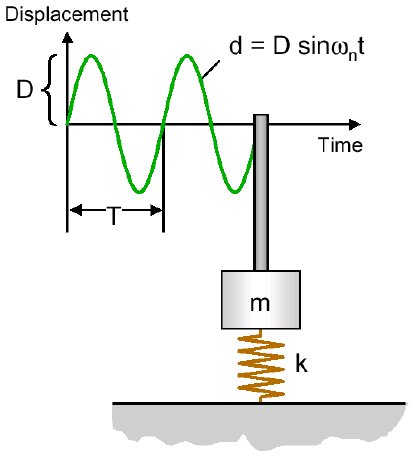
\includegraphics[scale=0.35]{ch1/2}
			\captionof{figure}{}
			\end{wrapfigure}		
			We can already get some definition, let's consider the free vibration assumed to be always in resonance. We can then define the \textbf{period of resonance} $T_n$, the \textbf{resonance frequency} $f_n = \frac{1}{T_n}$ and the \textbf{resonance pulsation}:
			\begin{equation}
			\omega _n = 2\pi f_n = \sqrt{\frac{k}{m}}.
			\end{equation}
			
			Notice that if we increase mass, the frequency decreases. 
			\\\\
			
			\begin{wrapfigure}[8]{l}{7cm}
			\vspace{-5mm}
			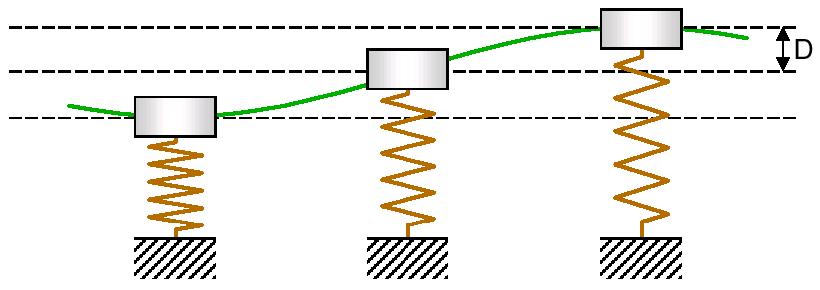
\includegraphics[scale=0.3]{ch1/3}
			\captionof{figure}{}
			\end{wrapfigure}
			Then we have the \textbf{energy transfer} between the kinetic energy and the potential energy. Indeed we see that velocity is null on extreme position and max when at the middle. This is written as:
			
			\begin{equation}
			\frac{1}{2} m V^2 = \frac{1}{2} kD^2
			\end{equation}
			
			where $V = 2\pi f_n D$. Replacing by this:
			
			\begin{equation}
			 m (2\pi f_n D)^2 = kD^2 \qquad \Rightarrow f_n = \frac{1}{2\pi}\sqrt{\frac{k}{m}}.
			\end{equation}
			
			We find a waited result. Now, let's show that \textbf{increasing damping reduces amplitudes over time}. Take the general newton equation for a linear free system and multiply by $\dot{x} (t)$:
			
			\begin{equation}
			m\ddot{x}\dot{x} + b\dot{x}\dot{x} + kx\dot{x} = 0 \qquad \Rightarrow \frac{d}{dt}\left( \frac{1}{2} m\dot{x}^2 + \frac{1}{2} kx^2 \right) = -b\dot{x}^2 \leq 0
			\end{equation}
			
	\section{Single degree of freedom oscillator}
		\begin{wrapfigure}[8]{r}{3.5cm}
			\vspace{-5mm}
			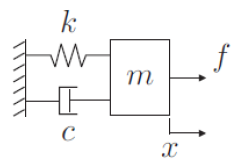
\includegraphics[scale=0.6]{ch1/4}
			\captionof{figure}{}
			\end{wrapfigure}
			Given the single degree system here, its free response is given by:
			
			\begin{equation}
			m\ddot{x}\dot{x} + b\dot{x}\dot{x} + kx\dot{x} = 0.
			\end{equation}
			
			We assume that this differential equation admits a solution of type $x = Ae^{st}$. We can then write the characteristic equation and its eigenvalues as:
			
			\begin{equation}
			ms^2 + cx + k = 0, \qquad s = - \frac{c}{2m} \pm j\sqrt{\frac{k}{m} -\frac{c^2}{4m^2}}.
			\end{equation}
			
			By defining two new quantity, the \textbf{natural pulsation} $\omega _n ^2 = \frac{k}{m}$ and the \textbf{damping ratio} $\xi$ such that $\xi \omega _n = \frac{c}{2m}$, we can rewrite:
			
			\begin{equation}
			s = - \xi \omega _n \pm j\omega _n \sqrt{1 -\xi ^2}.
			\end{equation}
			
			\begin{wrapfigure}[7]{l}{7.5cm}
			\vspace{-5mm}
			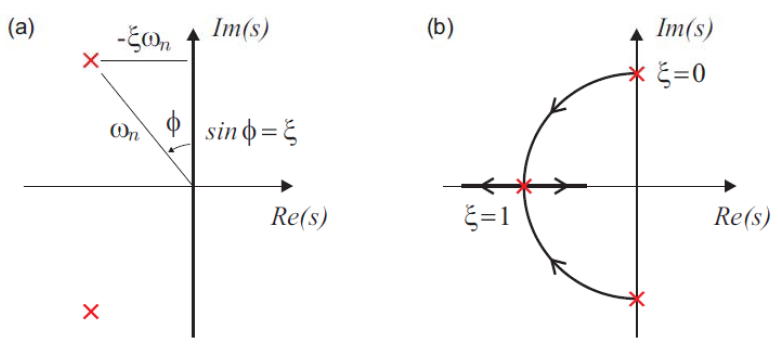
\includegraphics[scale=0.35]{ch1/5}
			\captionof{figure}{}
			\end{wrapfigure}
			We can introduce the \textbf{damping pulsation} $\omega _d = \omega _n \sqrt{1-\xi ^2}$. This explicitly makes appear the real and imaginary part of $s$ that we plot on a diagram. Notice that the norm and the angle of the complex number are $\omega _n$ and $\arcsin \xi$. \\
			
			The right figure is the \textbf{Nyquist diagram}. Last, the final expression for $x$ is:
			\begin{equation}
			x = e^{-\xi \omega _n t} \left( Ae^{j\omega _d t}+ Be^{-j\omega _d t} \right) = e^{-\xi \omega _n t} \left( A_1\cos (\omega _d t)+ B_1 \sin (\omega _d t) \right)
			\label{eq:1.8}
			\end{equation}
			where $A,B,A_1,B_1$ depends on initial conditions. 
			
			\subsubsection{Impulse response}
				\begin{wrapfigure}[9]{l}{2cm}
				\vspace{-5mm}
				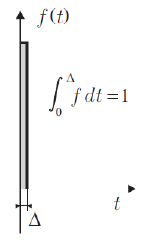
\includegraphics[scale=0.6]{ch1/6}
				\captionof{figure}{}
				\end{wrapfigure}
				Let's now apply an impulse on the system and let's analyse when it is applied during the infinitesimal time $\Delta$, given the initial conditions $x = 0, \dot{x}=0$. If we integrate the newton equation:
				\begin{equation}
				\int _0 ^\Delta m \ddot{x} \,dt = \int _0 ^\Delta f \,dt - \cancel{\int _0 ^\Delta c \dot{x}\,dt} - \cancel{\int _0 ^\Delta kx\,dt} = 1
				\end{equation}				 
				where the spring and damping forces cancel as they are finite (infinitesimal integral), the impulse integral =1 by definition. Taking the limit we find new initial conditions:
				
				\begin{wrapfigure}[8]{r}{3.5cm}
				\vspace{-5mm}
				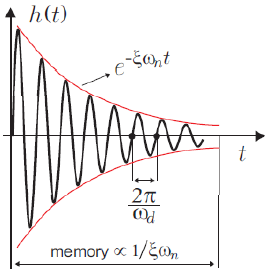
\includegraphics[scale=0.5]{ch1/7}
				\captionof{figure}{}
				\end{wrapfigure}
				\begin{equation}
				\lim _{\Delta \rightarrow 0} m\dot{x}(\Delta) = m\dot{x}(0^+) = 1  \qquad \Rightarrow x(0^+) = 0, \dot{x}(0^+) = \frac{1}{m}.
				\end{equation}

				The resolution of \eqref{eq:1.8} gives the \textbf{impulse response}:
				\begin{equation}
				x(t) = h(t) = \frac{1}{m\omega _d} e^{- \xi\omega _n t} \sin (\omega _d t)
\end{equation}				 

	\section{Convolution integral}
		\begin{wrapfigure}[8]{l}{4cm}
		\vspace{-5mm}
		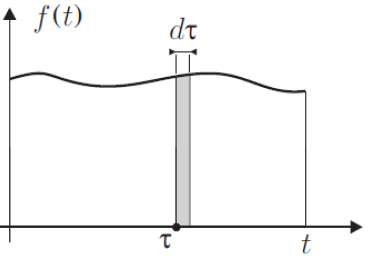
\includegraphics[scale=0.4]{ch1/8}
		\captionof{figure}{}
		\end{wrapfigure}
		Consider a transfer function $h(t)$ of a system and the decomposition shown on the figure. The output of the system will be computed with the convolution integral:
		
		\begin{equation}
		x = \int _0^t h(t-\tau)f(\tau) \, d\tau.
		\end{equation}
		
		In particular, for a \textbf{causal} system:
		
		\begin{equation}
		x(t) = \int _{-\infty}^{\infty} h(t-\tau)f(\tau)\, d\tau = \int _{-\infty}^{\infty} h(\tau)f(t-\tau)\, d\tau = h(t)*f(t).
		\end{equation}	
		
		\subsubsection{Harmonic response}
			Consider an undamped system	to which we apply an harmonic force:
			
			\begin{equation}
			m \ddot{x} + kx = F e^{j\omega t}.
			\end{equation}
			
			By considering the Fourier transform $x(t) = X(j\omega )e^{j\omega t}$, we get:
			
			\begin{equation}
			-\omega ^2 X(j\omega) + \frac{k}{m} X(j\omega) = \frac{F(j\omega)}{m} \qquad \Rightarrow X = \frac{F}{k} \frac{1}{1-(\omega / \omega)^2} = \frac{F}{k} D(\omega)
			\end{equation}
			
			where $D(\omega)$ is the \textbf{dynamic amplification}. For the damped case, we only have to know that $\xi \omega _n = c/2m$ and we get in the same way as previously:
			
			\begin{equation}
			X = \frac{F}{k}\frac{1}{1-(\omega / \omega)^2 + 2j\omega / \omega _n } = \frac{F}{k} D(\omega).
			\end{equation}
			
			The two dynamic amplification are plotted on the figures below, the second on a Bode diagram where we can clearly see the \textbf{Quality factor} defined as $Q = 1/2\xi$. 
			
			\begin{center}
			\begin{minipage}{0.4\textwidth}
			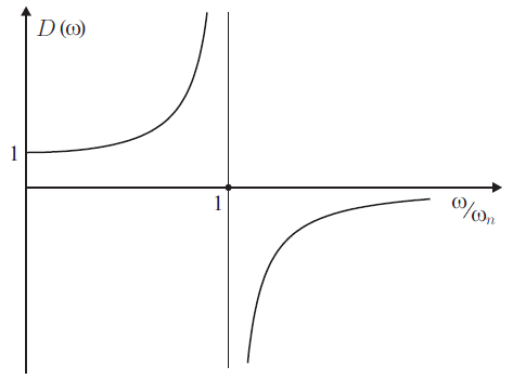
\includegraphics[scale=0.4]{ch1/9}
			\captionof{figure}{}
			\end{minipage}
			\begin{minipage}{0.4\textwidth}
			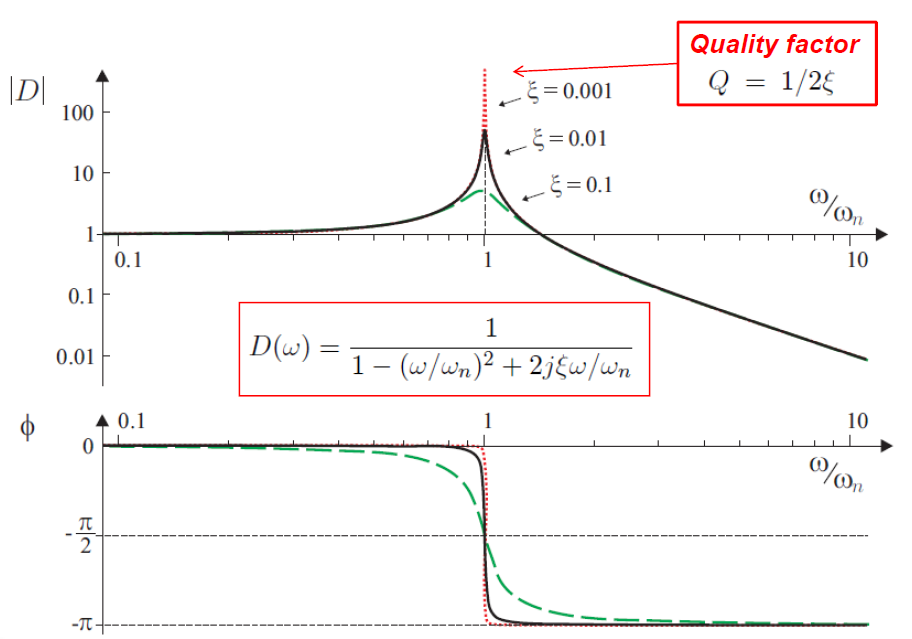
\includegraphics[scale=0.24]{ch1/10}
			\captionof{figure}{}
			\end{minipage}
			\end{center}